\documentclass[11pt,letterpaper]{article}

% \documentclass{article}
%    \usepackage{amsmath}
%    \usepackage{amssymb}
%    \usepackage{amsfonts}
%    \usepackage{graphicx}
%    \usepackage[mathscr]{euscript}
%    %\usepackage{bbm}
%    \usepackage[margin=1.0in]{geometry}
%    \usepackage{hyperref}
%    \usepackage{comment}
%    %\usepackage{todonotes}

%    %\usepackage{simplewick}
%    \usepackage{slashed}
%    %\usepackage{undertildeMod}

%    %\usepackage{feynmp-auto}
%    %\usepackage{youngtab}
%    %\usepackage[vcentermath]{youngtab}

%\usepackage{tikz}

%    \usepackage{enumitem}

    \newcommand{\vectsym}[1]{ \vec{#1} }
    %\newcommand{\vectsym}[1]{ \overline{#1} }
    %\newcommand{\vect}[1]{\vectsym{\boldsymbol{#1}}}
%    \newcommand{\vect}[1]{\boldsymbol{#1}}
    \newcommand{\vect}[1]{\vectsym{#1}}

    \newcommand{\udd}[2][]{{{\mathrm{d}^{#1}} #2}}
    \newcommand{\ud}[2][]{{ \, \udd[#1]{#2} \,}}
    \newcommand{\dd}[3][]{\frac{\udd{^{#1} #2 }}{\udd{ {#3}^{#1} }}}
    \newcommand{\uDD}[2][]{{{\mathcal{D}^{#1}} #2}}
    \newcommand{\uD}[2][]{{ \, \uDD[#1]{#2} \,}}
    \newcommand{\fdd}[3][]{{  \frac{ {\delta^{#1}}#2}{\delta #3} }}
    \newcommand{\vdd}[3][]{{ \fdd[#1]{#2}{#3}  }}
    %\newcommand{\pdd}[2]{ \frac{ \partial{#1} }{ \partial{#2} } }
    \newcommand{\limint}[2]{ \int\limits_{#1}^{#2} }
    \newcommand{\limintf}[4]{\limint{#1}{#2}\frac{#3}{#4}}
    \newcommand{\limintd}[3]{ \int\limits_{#1}^{#2}{\udd{#3}\,} }
    %\newcommand{\intd}[1]{ \int{\udd{#1}} }
    \newcommand{\intd}[2][]{ \int{\udd[#1]{#2}\,} }
    \newcommand{\intD}[2][]{ \int{\uDD[#1]{#2}\,} }
    \newcommand{\intdf}[3][]{\int\frac{\ud[#1]{#2}}{#3}}
    \newcommand{\intdff}[4][]{\int\frac{\ud[#1]{#2}#3}{#4}}
    \newcommand{\limintdf}[5][]{\limint{#2}{#3}\frac{\ud[#1]{#4}}{#5}}
    \newcommand{\limintdff}[6][]{\limint{#2}{#3}\frac{\ud[#1]{#4}#5}{#6}}

    \newcommand{\unit}[1]{\,\widehat{ \boldsymbol{#1} }}
    \newcommand{\paren}[1]{{\left( #1 \right)}}
    \newcommand{\bparen}[1]{\Bigl( #1 \Bigr)}
    \newcommand{\bbparen}[1]{\Biggl( #1 \Biggr)}
    \newcommand{\brac}[1]{\left[ #1 \right]}
    \newcommand{\bbrac}[1]{\Bigl[ #1 \Bigr]}
    \newcommand{\bbbrac}[1]{\Biggl[ #1 \Biggr]}
    \newcommand{\cbrace}[1]{{ \left\{ #1 \right\} }}
    \newcommand{\bcbrace}[1]{{ \Bigl\{ #1 \Bigr\} }}
    \newcommand{\bmat}[1]{  \begin{bmatrix}  #1  \end{bmatrix}   }
    \newcommand{\pmat}[1]{  \begin{pmatrix}  #1  \end{pmatrix}   }
    %\newcommand{\inv}[1]{\frac{1}{ #1 } }
    \newcommand{\ddsq}[2]{\frac{\udd^2}{\udd{ #2 }^2} #1 }
    \newcommand{\nline}[1]{\noindent\textbf{ #1 }}
    \newcommand{\nprob}[2]{\nline{ #1 } \begin{align*} #2  \end{align*} }
    \newcommand{\neqs}[2][*]{\begin{align#1} #2 \end{align#1}}
    \newcommand{\abs}[1]{\left| #1 \right|}
    \newcommand{\flux}[0]{\Phi}
    \newcommand{\del}[0]{\nabla}
    \newcommand{\vdel}[0]{\vect{\del}}
    \newcommand{\eval}[2]{\biggl|_{#1}^{#2}\biggr. }
    \newcommand{\smeval}[2]{\Bigl|^{#1}_{#2}\Bigr. }
    \newcommand{\pd}[1]{\partial #1}
    \newcommand{\pdd}[3][]{\frac{\pd{^{#1} #2 }}{\pd{ {#3}
    %^{#1}
    }}}
    \newcommand{\ang}[1]{\left\langle #1 \right\rangle}
    \newcommand{\expon}[1]{ \,\mathrm{e}^{ #1 } }
    \newcommand{\emf}[0]{\varepsilon}

    \newcommand{\bfrac}[2]{ \brac{\frac{ #1 }{ #2 }} }
    \newcommand{\pfrac}[2]{ \paren{\frac{ #1 }{ #2 }} }
    \newcommand{\ptfrac}[2]{ \paren{\tfrac{ #1 }{ #2 }} }
    \newcommand{\vud}[2][]{ \ud{#1\vect{ #2 }} }

    \newcommand{\ee}[1]{\times10^{#1}}
    \newcommand{\un}[1]{\,\mathrm{ #1 }\,}
    \newcommand{\ans}[3]{\, #1 \ee{#2} \un{#3} }
    \newcommand{\qty}[3]{\paren{\, #1 \ee{#2} \un{#3} }}
    \newcommand{\smqty}[2]{\paren{\, #1 \un{#2} }}
    \newcommand{\smans}[2]{\, #1 \un{#2} }

    \newcommand{\basis}[1]{ \,\unit{\mathrm{e}}_{ #1 } }
    \newcommand{\q}[1]{q_{#1}}
    \newcommand{\bq}[1]{\,\unit{\mathrm{q}}_{#1}}
    \newcommand{\be}[1]{\basis{#1}}
    \newcommand{\bbe}[2]{\be{#1}\be{#2}}
    \newcommand{\bep}[1]{\be{#1}'}
    \newcommand{\vectc}[3]{ \vectcc{#1}{+#2}{+#3} }
    \newcommand{\vectcc}[3]{#1 \basis{x} #2 \basis{y} #3 \basis{z} }
    \newcommand{\tensor}[1]{#1}
    \newcommand{\tp}[0]{\mathrm{T}}%transpose
    \newcommand{\infsum}[1]{ \sum_{n=0}^{\infty}{#1} }
    \newcommand{\dualsum}[1]{\infsum{}\sum_{k=0}^{n}{#1}}
    \newcommand{\qeq}[0]{\overset{?}{=}}
    \newcommand{\res}[0]{\,\mathrm{res}}
    \newcommand{\resw}[1]{\res\paren{w,#1}}
    \newcommand{\Four}[1]{\mathscr{F}\left\{ #1 \right\}}
    \newcommand{\invFour}[1]{\mathscr{F}^{-1}\left\{ #1 \right\}}
    \newcommand{\Heav}[0]{\,\mathrm{H}}
    \newcommand{\heav}[0]{\Heav}
    \newcommand{\delt}[0]{\,\delta}
    \newcommand{\infint}[0]{\int_{-\infty}^{\infty}}
    \newcommand{\infintd}[1]{\infint\ud{#1}}
    \newcommand{\conv}[0]{\otimes}
    \newcommand{\scr}[1]{\mathscr{#1}}
    \newcommand{\Lap}[1]{\mathscr{L}\left\{ #1 \right\}}
    \newcommand{\invLap}[1]{\mathscr{L}^{-1}\left\{ #1 \right\}}
    \newcommand{\iif}{\quad \mathrm{if}\,}

    \newcommand{\pw}[2][cc]{\left\{ \begin{array}{#1} #2 \end{array} \right. }

    \newcommand{\pcos}[1]{\cos{\paren{#1}}}
    \newcommand{\psin}[1]{\sin{\paren{#1}}}

    \newcommand{\uu}[1]{\underline{#1}}
    \newcommand{\eq}[2][\notag]{\begin{equation}#1 #2 \end{equation}}
    \newcommand{\enum}[1]{\begin{enumerate} #1 \end{enumerate} }
    \newcommand{\bitem}[1]{\item[\textbf{#1}]}
    \newcommand{\bbitem}[2]{\item[\textbf{#1}] (#2)\,}

    \newcommand{\ffrac}[3][]{{ #1{\frac{#2}{#3}} }}
    \newcommand{\poissonbrac}[1]{ {\left\{ #1 \right\}} }
    \newcommand{\bars}[1]{{\left| #1 \right|}}
    \newcommand{\detmat}[1]{\begin{vmatrix} #1 \end{vmatrix}}
    \newcommand{\qtq}{\quad\to\quad}
    \newcommand{\qTq}{\quad\implies\quad}
    \newcommand{\opdot}[1]{\overset{\scriptscriptstyle \circ}{#1}}
    \newcommand{\opddot}[1]{\overset{\circ\circ}{#1}}

	\newcommand{\enumb}[1][]{\begin{enumerate}[#1]}
    \newcommand{\enume}{\end{enumerate}}

    \newcommand{\rr}{\vect{r}}
    \newcommand{\R}{\mathbb{R}}
    \newcommand{\Z}{\mathbb{Z}}

    \newcommand{\upperlower}[3]{{ {#1}^{#2}_{\phantom{2}#3} }}
    %\newcommand{\ul}[3]{\upperlower{#1}{#2}{#3}}
    \newcommand{\lowerupper}[3]{{ {#1}_{#2}^{\phantom{2}#3} }}
    %\newcommand{\lu}[3]{\lowerupper{#1}{#2}{#3}}

    \newcommand{\ket}[1]{{ \left | #1 \right \rangle }}
    \newcommand{\bra}[1]{{ \left \langle #1 \right | }}
    \newcommand{\bk}[2]{{ \left \langle #1 \middle | #2 \right \rangle }}
    \newcommand{\bok}[3]{{ \left \langle #1 \middle | #2 \middle | #3 \right \rangle }}
    \newcommand{\bo}[2]{{ \left \langle #1 \middle | #2 \right .}}
    \newcommand{\ok}[2]{{ \left . #1 \middle | #2 \right \rangle}}
    \newcommand{\kb}[2]{{ \ket{#1}\bra{#2} }}

    \renewcommand{\a}[1][\vphantom{\dagger}]{{a^{#1}}}
    \newcommand{\ad}{\a[\dagger]}
    \newcommand{\kk}{{k\vphantom{k'}}}
    \newcommand{\kp}{{k'}}
    \newcommand{\kpp}{{k''}}
    \newcommand{\comm}[2]{\brac{\,#1\,,\,#2\,}}
    \newcommand{\acomm}[2]{\cbrace{\,#1\,,\,#2\,}}
    \renewcommand{\L}{\scr{L}}
    \newcommand{\inv}{^{-1}}
    \newcommand{\norder}[1]{\,: #1 :\,}
    \newcommand{\obar}[1]{{ \overline{#1} }}
    \newcommand{\wick}[6][1]{{ \contraction[#1 ex]{#2}{#3}{#4}{#5} #2#3#4#5#6}}
    \newcommand{\sq}{^{\,2}}
    \newcommand{\fcn}[1]{{\,\mathrm{#1}\,}}
    \newcommand{\op}[1]{\widehat{#1}}
    \newcommand{\tr}{\fcn{tr}}
    \newcommand{\Tr}{\fcn{Tr}}
    \newcommand{\T}{\fcn{T}}

    \newcommand{\lra}{\leftrightarrow}
    \newcommand{\nothing}[1]{}
    \newcommand{\half}[1][1]{ {\frac{#1}{2}} }
    \newcommand{\thalf}[1][1]{ {\tfrac{#1}{2}} }
    \newcommand{\id}{ {\mathbf{1}} }
    \newcommand{\sigmab}{ {\bar{\sigma}} }
    \newcommand{\dg}{ {\dagger} }
    \newcommand{\pdg}{ {\vphantom{\dagger}} }
    \newcommand{\gr}[1]{ {\mathrm{#1}} }

    %\DeclareSymbolFont{bbold}{U}{bbold}{m}{n}
    %\DeclareSymbolFontAlphabet{\mathbbold}{bbold}

    \newcommand{\kd}[2]{{ \delta^{#1}_{#2}}}
    \newcommand{\kdu}[1]{{ \delta^{#1}}}
%    \newcommand{\Sl}[1]{{{ S_{#1}}}
%    \newcommand{\Su}[1]{{{ S^{#1}}}
%    \newcommand{\Smat}[4]{{{ (S_{#1#2})^{#3#4}}}
%    \newcommand{\kdg}[4]{{{ \kd{#3}{#1}\kd{#4}{#2}}}
%    \newcommand{\kdgg}[4]{{{ \kd{#4}{#1}\kd{#3}{#2}}}
%    \newcommand{\Smatd}[4]{{{ \kdg{#1}{#2}{#3}{#4}-\kdgg{#1}{#2}{#3}{#4}}}
%    \newcommand{\Smatdp}[4]{{{ \big(\Smatd{#1}{#2}{#3}{#4}\big)}}
%    \newcommand{\g}[1]{g_{#1}}
%    \newcommand{\gu}[1]{g^{#1}}
%····
    \newcommand{\ub}{\overline{u}}
    \newcommand{\vb}{\overline{v}}
    \newcommand{\gv}{\gamma^5}
    \newcommand{\gm}[1]{{\gamma^{#1} }}
%    \newcommand{\Tr}[1]{\,\mathrm{Tr}\brac{#1}}
    \newcommand{\ps}{\slashed{p}}
    \newcommand{\ks}{\slashed{k}}
    \newcommand{\pds}{\slashed{\pd}}
    \newcommand{\psib}{\bar{\psi}}

%    \newcommand{\ul}[3][]{#1^{#2\phantom{#3}}_{\phantom{#2}#3} }
    \newcommand{\ulul}[5][]{#1^{#2\phantom{#3}#4\phantom{#5}}
                            _{\phantom{#2}#3\phantom{#4}#5} }
    \newcommand{\symindBinU}[5]{ {#1}^{#2#3}{#1}^{#4#5} 
                                    + {#1}^{#2#4}{#1}^{#3#5}
                                    + {#1}^{#2#5}{#1}^{#3#4} }
    \newcommand{\symindBinL}[5]{ {#1}_{#2#3}{#1}_{#4#5} 
                                    + {#1}_{#2#4}{#1}_{#3#5}
                                    + {#1}_{#2#5}{#1}_{#3#4} }
    \newcommand{\gindBinU}[5]{ {#1}^{#2#3}{#1}^{#4#5} 
                                    - {#1}^{#2#4}{#1}^{#3#5}
                                    + {#1}^{#2#5}{#1}^{#3#4} }
    \newcommand{\gind}[4]{\gindBinU{g}{#1}{#2}{#3}{#4} }
    \newcommand{\tot}{\leftrightarrow}
    \newcommand{\diag}{\fcn{diag}}
    \newcommand{\itemb}{\begin{itemize}}
    \newcommand{\iteme}{\end{itemize}}

    \newcommand{\newQuestion}[2]{ \section*{Question #1 \textnormal{: #2 } } }
    \newcommand{\hc}{ {\text{h.c.}} }
    \newcommand{\ptext}[1]{\paren{\text{#1}}}

    \newcommand{\set}[1]{ \cbrace{#1} }
    \newcommand{\lie}[3][]{ {{\mathrm{#2}}_{#1}\paren{#3} } }

    \newcommand{\lag}{ {\mathcal{L}} }
    \newcommand{\Lag}{ \lag }
    \newcommand{\amp}[1][M]{ {\mathcal{#1}} }
    \newcommand{\Amp}[1][M]{ \amp[#1] }

    \newcommand{\p}{\vect{p}}

    \newcommand{\fig}[2][]{
	    \begin{figure}[#1]\begin{center}
		    #2
	    \end{center}\end{figure}
    }



% filename: PhysMan.tex

%% FOR Sans Serif UNCOMMENT THE FOLLOWING TWO LINES
%\usepackage[T1]{fontenc}
%\renewcommand*\familydefault{\sfdefault} %% Only if the base font of the document is to be sans serif
%% (To get normal Serif font again, comment the two lines)


%----------------------------------------------------------------
% Attempts at changing the font to sans serif style
%----------------------------------------------------------------

% http://www.tug.dk/FontCatalogue/sansseriffonts.html

%%\usepackage[light,math]{iwona}
%%\usepackage[T1]{fontenc}

%%\usepackage{cmbright}
%%\usepackage[T1]{fontenc}

% Works:
%\usepackage[T1]{fontenc}
%\renewcommand*\familydefault{\sfdefault} %% Only if the base font of the document is to be sans serif

%%\usepackage[default]{sourcesanspro}
%%\usepackage[T1]{fontenc}



%----------------------------------------------------------------
% Other style options
%----------------------------------------------------------------

\usepackage{fullpage}
\usepackage{graphicx}
\usepackage{amsmath}
\usepackage{amssymb} % Math symbols such as \boldsymbol

\usepackage{fancyhdr}
\pagestyle{fancy}
%\fancyfoot[C]{\thepage}
\usepackage[
%  margin=2.5cm,
  left=2.5cm, right=2.5cm,
  top=2cm, bottom=2cm,
  includefoot,
  footskip=30pt,
  headsep=1.25cm % Seperate header and main body by
		% headsep -- prevents first line from overlaying on top of header
]{geometry}

\usepackage[noams,squaren,Gray]{SIunits} % Standardizes quantity and SI unit spacing
\usepackage{soul} % for an underline macro that wraps
 \setul{0.2ex}{.4pt}% underline 0.2ex below contents
\usepackage{enumitem} % for enumerate options
\usepackage{verbatim} % Allows display of almost any sequence of symbols, printed in typewriter font; and provides comment environment
\usepackage[obeyspaces,spaces]{url} % Same as verbatim but allows line breaks and spaces
\usepackage{parskip}
 \setlength{\parindent}{0em}
 \setlength{\parskip}{2.2ex}

%\usepackage[compact]{titlesec}
%\titlespacing{\section}{0pt}{*1ex}{*0.5ex}
%\titlespacing{\subsection}{0pt}{*0}{*0}
%\titlespacing{\subsubsection}{0pt}{*0}{*0}
\usepackage{titlesec}
\titlespacing{\subsection}{0pt}{*2.5}{*0.1}



%----------------------------------------------------------------
% Macros
%----------------------------------------------------------------

% Scientific Notation and Units
% =============================

% scientific notation without units
\providecommand{\sn}[2]{ {#1} \mkern-1.5mu\times\mkern-3mu 10^{#2} }
% scientific notation with units
\providecommand{\snu}[3]{ \unit{\sn{#1}{#2}}{#3} }

% create compact or ``squished'' lists with sublists:
\newcommand{\squishlist}{
   \vspace{-2.2ex}
   \begin{list}{$\bullet$}
    { \setlength{\itemsep}{0pt}      \setlength{\parsep}{3pt}
      \setlength{\topsep}{3pt}       \setlength{\partopsep}{0pt}
      \setlength{\leftmargin}{1.5em} \setlength{\labelwidth}{1em}
      \setlength{\labelsep}{0.5em} } }
\newcommand{\squishend}{
    \end{list}  }

% struts for spacing in tabulars/tables
\newcommand{\tstrut}{\rule{0pt}{2.5ex}}
\newcommand{\bstrut}{\rule[-1ex]{0pt}{0pt}}
\newcommand{\Tstrut}{\rule{0pt}{2.9ex}}
\newcommand{\Bstrut}{\rule[-1.4ex]{0pt}{0pt}}


\usepackage{todonotes}
%\graphicspath{{../../imgs/6labs/6Alab/6Aexp6/}}
\graphicspath{{../../}}

\usepackage{hyperref}
\hypersetup{
    colorlinks=true,
    linkcolor=blue,
%    filecolor=magenta,      
%    urlcolor=cyan,
}

\usepackage{color}		% Text color
\usepackage{xspace}  	% Space at end of macros


%\newcommand{\TODO}[2][inline,color=green!40]{{ \todo[#1]{#2} }}
\newcommand{\TODO}[2][inline,color=green!40,caption={}]{{ \todo[#1]{#2} }}
%\newcommand{\TODOdefaultNotColor}{inline,caption={}}
%\newcommand{\TODOdefaultColor}{color=green!40}
%\newcommand{\TODO}[2][\TODOdefaultNotColor,color=green!40]
%	{{\todo[#1]{#2}}}
%\newcommand{\TODOg}[2][\TODOdefaultNotColor]{ \todo[color=green!40,#1]{#2} }
\newcommand{\TODOg}[2][inline,caption={}]{ \todo[color=green!40,#1]{#2} }
\newcommand{\TODOshanna}[2][inline,caption={}]
		{ \todo[color=red!40,#1]{\shanna{} #2} }
\newcommand{\TODOmeeting}[2][inline,caption={}]
		{ \todo[color=blue!40,#1]{\meeting{} #2} }
%\newcommand{\question}[2][]{{ \bf #2 }}
\newcommand{\question}[2][blue]{\textcolor{#1}{#2}}

%\newcommand{\qq}[2][]{{ \question }}

\newcommand{\answer}[2][red]{\textcolor{#1}{#2}}

\newcommand{\action}[2][]{ #2 }

%%	Decide whether to refer to vertical intercept (a) as such; 
%%		(b) as $y$-intercept; or (c) as $B$-intercept.
%\newcommand{\yint}[1][B]{$#1$-intercept }
%\newcommand{\yint}[1][y]{$#1$-intercept }
\newcommand{\yint}[1][]{vertical intercept\xspace}

\newcommand{\itm}[2][\\ * ]{#1#2}

\newcommand{\temp}[2][]{#1#2}

% indicate that Shanna made a comment
\newcommand{\shanna}[1][]{{\bf Comment from Shanna:}\xspace}
% indicate a comment was introduced at a meeting
\newcommand{\meeting}[1][]{{\bf Comment from meeting:}\xspace}


%% Compile controls
%%		If the following lines are uncommented, the corresponding 
%%		text features will be turned off.  Questions will be displayed
%%		in normal font, while answers and todo notes will be turned off.

%\renewcommand{\question}[2][]{#2}
%\renewcommand{\answer}[2][]{}
%\renewcommand{\TODO}[2][]{}
%renewcommand{\temp}[2][]{}


\begin{document}

\fancyhead[C]{Physics 6A Lab \rule[-1ex]{0pt}{0pt}\(\mid\) Experiment 6}
%\fancyhead[C]{Physics 6A Lab \rule[+1ex]{5pt}{5pt}\(\mid\) Experiment 6}

\vspace{-5ex}
\part*{Rewritten Biceps Lab}
\TODO{
	LEGEND:\\
	* [Black text] -- Regular text \\
	* \question{Question or action the students need to take
		(Mostly for ease of instructor understanding)} \\
	* \answer{Tip for TAs or answer to student question.  
	Will be removed from student verstion of the lab.}
	\\
	* [These green or orange boxes]
	-- comments on what needs to be done, etc.  
Not part of the lab for students.
}


\TODO{Overall TODO list:  (In addition to items scattered throughout the text)
	\\
	{\bf More practical considerations}
	\itm Actually write the warm up problems
	\itm Replace $\alpha$ with $90\degree-\theta$, and add $\theta$ to diagrams,
	in order to emphasize connection to the angle usually 
	referenced in torque calculations.
	\itm {{\bf Just tell them the model is linear}}
	\itm Consider guiding students through derivation of
	$B$ vs $H$ equation.  
	(Note that there's a question at the end which almost gets there, 
	and requires students to think critically about the derivation.)
	\itm Supplement pictures of apparatus with biological pictures.  Possibly
	ask students to do fill-in-the-blanks for both sets of pictures.
	\itm Ask students to estimate the `experimental parameters' associated
	with their own arms.  Maybe ask how the force compares for someone with a
	shorter arm.
	\answer{$R,r,W$ all smaller, $H,\theta$ remain the same.
		Less torque due to bicep, but also less torque due to hand force
		and weight of arm.  
		If $r$ and $R$ decrease in proportion, it takes the smaller person
		slightly less biceps force to lift the same amount of weight.
	}
	\\
	{\bf More on the meta side}
	\itm Be careful (and consistent) with word choice.  
			E.g.: parameters, models, formulas.
	\itm Think about specific learning outcomes
	\itm Think about how well lab accomplishes learning goals/outcomes
	\itm Make the procedure easier for students to read 
	-- break into numbered bullet points
	\itm Consider creating sample sheet on which to write data, or just a list
	of all the specific tasks the students need to perform.  Note that this list
	might work well while I'm overseeing this lab, but future TAs will likely
	want to modify it.
}

\TODO{(Rough) {\bf Learning goals}
	-- gain familiarity with/understanding of the following:
	\itm Basic static torque -- distance and magnitude of force
	\itm Angle in torque -- make sure to really emphasize this
	\itm Torque applies to human arm
	\itm Biceps force is linear in force on hand
	\itm Emphasis on what a linear model looks like
	\itm Understad what it's like to apply a theoretical model
	to a complicated real-world situation (like a human arm).
	Understand that this will [always] be an approximation, 
	and that we need to figure out how good an approximation our model is.
}

\TODOshanna{
	Add these to main text:\\ 
	``By the end of this lab, you will be able:\\
1. Describe how torque depends on applied force and distance 
of force from pivot point.\\
2. Determine how angle of applied force increases or decreases applied torque\\
3. Use concepts of torque to understand aspects of human arm.\\
4. Relate bicep muscle force to weight lifted by hand.\\
5. Extrapolate linear model to make predictions?\\
6. Recognize the benefits and limitations of a applying a basic
physics model to a real-world situation (like a human arm).''\\
Adjust wording to reflect what was in lab learning outcomes
document, if possible.
Only include those that explicitly ask the student to show these
by answering a question.
}

\TODO{Some notes on word choice:\\
	{\bf Still deciding}
	\itm Experimental parameters
	\itm Parameters vs coefficients in equations
	\itm Formula vs equation vs function
	\itm Apparatus vs experimental setup
	\itm Real world situation vs application vs ?
	\\
	{\bf Decided upon (though subject to discussion)}
	\itm `Model' will always refer to a mathematical model.
	Distinguish between experimental models [experimentally determined models]
	and theoretical models
	\itm Vertical intercept, vs y-interecept or B-interecept
}


\temp{\pagebreak}
\section*{Introduction}

\TODOshanna{
	Recommend emailing students in advance to get them excited. :)
	Add something like ``Because it generally takes longer to devise your own
	steps, you will notice this lab has significantly fewer parts.''
}
	

This lab will be different from the others you've done so far.
First, we'll have some warm-up exercises to familiarize yourself 
with some of the theory, as well as the experimental setup.
Then you'll move on to the experiment itself.

Rather than giving you explicit steps to follow at every stage,
at times we'll provide you with a problem to investigate
and some hints on how to proceed.  
It will be something of a challenge to figure out how exactly to accomplish
each step, but this will be much more like doing science in the real world.
We hope you enjoy the process!


\subsection*{Warm up}
\TODO{
	{\bf Comments on warm up:}
	\itm Assume students don't know anything about torque
		(it's very likely they won't know anything)
	\itm Give activity which guides them through torque
	\itm Possibly just take from open source tutorial
	\itm Ok, open source tutorial requires them to do experiment that we don't
		have resources set up for 
		(though we could relatively easily set them up, 
		especially in a future quarter)
}
\TODOshanna{Mastering physics may have a good activity}

\subsubsection*{Warm up I:  Torque}

\TODO{A lot of these problems can be taken with minimal modification
	from the UMD open source 
	\href{https://www.dropbox.com/sh/i3iftgdflca6yj0/AAA37zsDuMN591__i-oPnjiSa/Suite\%20II/Instruction/Student_Materials/01_Torque/Tutorial_01_Torque.doc?dl=0}
		{tutorial on torque} 
		(and the 
		\href{https://www.dropbox.com/sh/i3iftgdflca6yj0/AABuUrEqKUU4ZvRvxi_cQLWYa/Suite\%20II/Instruction/Student_Materials/01_Torque/Tutorial_01_Homework.doc?dl=0}
		{corresponding HW assignment}
		) [click colored text for links], which focus on static torque ,
		especially on things like levers
}
\TODO[inline]{Note:  These questions would probably work better if
	the students could actually perform 
	some of these mini-experiments.
	I'm planning to talk to those in charge (not Marty, but others)
	to ask whether we have the materials needed to investigate 
	the balance of torques on a simple lever-fulcrum system
	(like the one in the 
	\href{https://www.dropbox.com/sh/i3iftgdflca6yj0/AAA37zsDuMN591__i-oPnjiSa/Suite\%20II/Instruction/Student_Materials/01_Torque/Tutorial_01_Torque.doc?dl=0}
	{open source tutorial activity}
	).
	{\bf Such an apparatus will not be available this quarter, but it may
	work for next quarter} -- 
	depending on the resources already in place.
}
\TODO[inline,color=green!40,caption={}]{
{\bf Outline of some warm-up questions}
\enumb
	\item Balancing weights on a ruler atop a fulcrum
		\enumb[label=\alph*.]
			\item Two equidistant weights on opposite side of pivot
			\item Double one weight's distance; ask how much weight needs to be
				added and to which side
		\enume
	\item Replace one of the weights with an arbitrary force pointing downward
	\item Replace arbitrary force with a cable at an angle 
		(positioned like bicep)
\enume
}

\TODO{
	Need to figure out how to introduce quantitative relations\\
	* $\tau \sim rF$ (for orthogonal force) \\
	* $\tau \sim rF\sin\theta$ \\
}
\TODO{
Ideally, we'd have a simple mini-experiment for them to play with,
to help this introduction to torque.
This is almost certainly possible for a future quarter. 
}
\TODOshanna{Make two versions of this lab -- for this and next quarter}

\subsubsection*{Warm up II: The apparatus}
Before we get into equations, take a moment to understand the equipment.  
	Fill in the blanks on the diagram below, from among the following choices:
	upper arm (humerus), elbow, forearm, hand, and biceps muscle.
\TODO{TODO -- Block out the labels in the picture of the apparatus,
	and replace with blanks -- 
	similar to a diagram one might fill in for a biology
	course.  Blanks include 
	upper arm (humerus), elbow, forearm, hand, and biceps muscle.
}
\TODO{
	Do something similar for extended free body diagram (?)
}
\TODOmeeting{
\itemb
	\item Have them fill in the same diagram with forces and distances, 
		given a description of those forces/distances in words.
		\subitem They'll be given a rectangle with some holes,
		and diagonal lines to give the appropriate angle for the 
		upper arm and biceps
		\subitem Have $W$ on diagram already, mentioning center of mass
		\subitem Label $\theta$ already
	\item Fix pivot point in diagram (doesn't currently line up)
\iteme
}

\begin{figure}[h!]
	\centering
	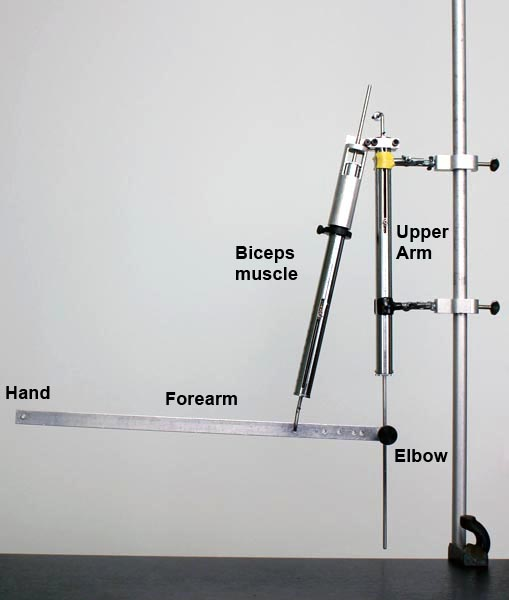
\includegraphics[width=0.6\textwidth]
	{{/imgs/6labs/6Alab/6Aexp6/6a-exp6_fig1_text_fix.jpg}}
\end{figure}
\begin{figure}[h!]
	\centering
	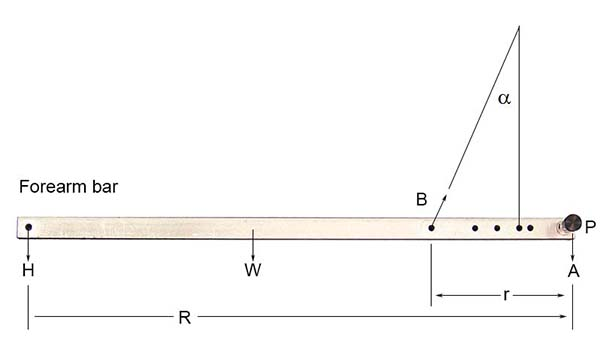
\includegraphics[width=0.6\textwidth]
	{{/imgs/6labs/6Alab/6Aexp6/6A_6_arm.jpg}}
\end{figure}


\TODO{
	Potential question for students:
	\textcolor{purple}{\bf \\
		\shanna
		Probably not worth the confusion this will cause.
		Just tell them how to deal with the scale as is. \\}
	The biceps force gauge is labeled in kilograms.  
	Strictly speaking, does this make sense?
	In particular, would this be correct if we used the gauge on the moon?
	What units should the scale be labeled with instead?
	Can you think of any reasons why it might be useful to have the scale
	labeled in kilograms?
}

\temp{\clearpage}
\section*{Procedure}
We wish to investigate some of the forces involved with weight lifting.
Specifically, we'll examine the situation where you're holding a weight in your
hand, with your forearm being held horizontal.
We'll measure the forces exerted by the biceps muscle.

If you'd like, imagine yourself as a 
physical therapist or prosthetic limb designer,
who wishes to combine physics with some 
general experimental design skills to determine 
some of the forces involved in lifting objects.

\TODO{TODO:  Common sense warning about using reasonable values, 
making sure to keep everything but the thing you're measuring constant, etc.}

%\TODO{ Discussion about which variables are relevant.  
%Answer -- forces, distances, angles. 
%Not sure whether to move this elsewhere}

\TODO{TODO: Make sure to emphasize that we'll keep the forearm horizontal, 
to simplify things.}

\question{Start by measuring the biceps force $B$ 
for some fixed weight $H$ being held in the hand.}
\TODOshanna{Tell them to record the values.}

Then devise and carry out a procedure for measuring the forces $B$ for
different weights $H$.  
\question{Make sure to explicitly write out the steps of the procedure.}
If you find you need to modify the procedure as you carry it out,
that's okay -- but be sure to change the written version to correctly
reflect the steps you really carried out.

After taking several measurements (you can choose a number which seems
reasonable), use your data to 
\question{extrapolate a relationship between the biceps
force $B$ and the weight $H$ in the hand.}
\TODOshanna[inline,fancyline]{Remind them ``You did this in the XX lab''}
\question{Write an explicit formula for $B$ as a function of $H$.}
\emph{Hint:  In case this terminology is a bit unfamiliar, 
it might help to know that
$y(t) = \bparen{10\,\mathrm{m}} +\bparen{4.9\,\mathrm{m/s^2}}t^2$ 
is an example of an explicit formula 
for $y$ as a function of $t$ (for a certain physical situation).}
Make sure you specify the units of the quantities.
\answer{The idea is that they need to realize to make a graph to do this.
	Then they need to notice that the graph is linear,
	so the `formula' is just the equation of a line.
}

Choose a new value for $H$ -- one that you haven't measured yet,
but that you are able to measure.  
Before you measure $B$, 
\question{use your model to predict the biceps force $B$ 
for this new value of $H$.}
\TODOshanna{``Before you make the measurement, 
have your TA approve your prediction and reasoning.''}

Now use the apparatus to measure $B$ for this value of $H$.  
\question{How does it compare to the prediction from your model?  }
(Calculate the percent deviation.)
If the two values don't exactly agree, do
you think this is okay?  
\question{Do you think it tells us our model is wrong?}
Why or why not?




\subsubsection*{Varying model parameters}
\TODO{TODO: Expand this prompt}
Using a combination of your intuition for how your own arm works,
and the knowledge of torque you developed in the warm up exercises,
\question{predict how the biceps force change when we increase 
each of the following parameters. }
Fill in your own copy of the chart below, 
answering with ``increases'', ``decreases'', 
``stays constant'', or ``something else''.  
(If you choose something else, explain why you chose that.)
\vspace{.5cm}
\\
\begin{tabular}{|c||c|c|c|}
	\hline
	Parameter change & Effect on $B$ & Effect on slope of graph &
	Effect on \yint  of graph \\ \hline \hline
	$\uparrow R$ 
	& & & 
	\\ \hline
	$\uparrow r$ 
	& & & \\ \hline
	$\uparrow W$ 
%	& & & \\ \hline
%	$\uparrow \alpha$
	& & & 
	\\ \hline

\end{tabular}
\TODOmeeting{
\itemb
	\item Replace slope with ``$\Delta B/\Delta H$'' and intercept with
		``value of $B$ when $H=0$''.
	\item Ask them whether these quantities correspond to anything on their
		graph
\iteme
}
\TODO{We're implicitly telling the students here that the data should be linear.
	This is perhaps not ideal, 
	but it makes questions like this one much less awkward and
	much more straightforward.
	\\
	Liz pointed out that nonlinear graphs still have slopes and intercepts,
	so technically we're not giving linearity away completely.
	At least not yet.
}
\TODO{
	Consider having students come up with their own ideas 
	of what parameters to vary.  
	Maybe only provide 3 lines.  
	Note that they might have trouble
	coming up with parameters other than $r$.  
	(Hopefully $r$ will be easy.)
}

The way our apparatus is set up, 
The easiest of the above parameters to vary is $r$.
Devise an experiment to 
\question{determine the effect that increasing $r$
has on the biceps force $B$ as well as 
on the slope and the \yint  of the graph.}
\answer{They should choose a new value for $r$, then re-enact their procedure
	to determine $B(H)$ for this new $r$ value.  
	{\bf It might be difficult for them
	to realize that they don't want to find $B(r)$ }
	-- doing so does answer the first question, 
	but it doesn't tell them anything about the slope or the \yint.}
\TODO{
	Subtlety: 
	Changing $r$ changes $\alpha$ as well.  This might be worth a footnote
		(or mills), but I won't lose any sleep over it, and it won't 
		much affect the data.
	{\bf If we really want to emphasize the importance of the angle
		at which the force is applied, we probably want to address this more
	than is already done.}
}




\begin{comment}
%% Section talking somewhat abstractly about models and asking for predictions.
	%% Likely difficult for students to comprehend, and likely will take too
	%% given the time constraints.
{{{
\subsubsection*{Extrapolate further}
The model you extrapolated from your data is a good description of the 
force $B$ on this apparatus for this setup.  But what if you change the
apparatus somehow?  For example, consider an apparatus which
is the same as yours, except the forearm bar is longer.
For the same value of the weight $H$ in the hand, 
would the corresponding biceps force $B$ change? 
In fact, it does: $B$ is larger for a larger value of $R$ 
(assuming all other parameters are left the same).
\TODO{Ideally ask them a question, to make sure they pay attention to
this part.}

In reality, you probably want a model of the biceps force that is valid 
beyond your specific apparatus.  
To do this, we'll try to determine the coefficients in your formula for 
$B(H)$ in terms of various parameters of your apparatus -- that is, in terms of
things you can actually measure!  
For example, one such parameter is the length of the forearm bar -- if you
change this parameter, the coefficients in the formular for $B(H)$ change.
\TODO{Subtelty -- three types of experimental parameters:  
	(1) independent/dependent variables, 
	(2) parameters which change model parameters, but not the form of the model
	(3) parameters which ``break'' the model 
		-- i.e., they change the form of the model.
	In this case, $r,R,\alpha,W$ are type (2), whereas the angle of the forearm
	to the horizontal is type (3).\\

	We might be able to get this across by giving them an extended worked
	example of another model -- for example, a simple static torque problem,
	like in the warm up.
}
}}}
\end{comment}

\subsubsection*{Understanding model parameters}
\TODO{
Ideally we'd have enough time to guide the students in deriving this formula,
but this isn't out main goal for the lab.  Hopefully we'll still give them some
intuition for the formula.
}

In a previous step above,
you experimentally determined a formula for the biceps force $B$ as a function
of the weight $H$ in the hand.  
Now we'll compare this model to the one the theory predicts.

It turns out that we can analyze the torques acting on the forearm
to determine a formula for $B$ vs $H$.  You actually have all the tools needed
to do this from the warm up exercises at the beginning of this lab, and we
encourage you to give it a try!  But in the interest of time, we'll just
provide you with the formula, which is as follows:
\begin{equation*}
	B = \paren{ H + \frac{W}{2} }\frac{R}{r\cos\alpha}
\end{equation*}

\begin{comment}
{{{
Given this theoretical model, 
can you determine what the theory predicts the coefficients appearing in
your formula for $B$ vs $H$ should be?  
Hopefully, you noticed your data plot of $B$ vs $H$ was linear.
It turns out, we can use the theoretical model to predict what the slope and
\yint  of that graph should be.
\question{First write your answer in terms of symbols} 
(i.e., variables) only;
\question{then, plug in the values for those variables} 
according to your apparatus, 
to determine the theoretical model coefficients.
How do these theoretical coefficients compare to your experimental model
coefficients?  
(\question{Calculate the percent difference} 
and \question{comment on how well they agree}.)

You just used a theoretical model to predict the values of your experimental
model coefficients.
Now, we'll look at the predictions the theoretical model makes on your data
itself.  
(This may seem similar to the previous step,
but there's actually a subtle difference.)
}}}
\end{comment}

%Hopefully, you noticed your data plot of $B$ vs $H$ was linear.
Now that we have this theoretical model, 
we can use it to predict what the slope and \yint of your graph should be.
First, use the theoretical model to 
\question{predict the slope and \yint  
of your graph in terms of symbols} (i.e., variables) only.
Next, \question{plug in the actual parameter values 
that correspond to your experimental apparatus}
to get a numerical value for these theoretical coefficients (with units!).
\question{How does this prediction compare 
with your actual slope and \yint ?}

\question{Do the theoretical predictions above agree 
with the predictions you recorded in the chart above},
regarding how the biceps force and linear equation parameters change when
increasing certain apparatus parameters?

\begin{comment}
You probably noticed some similarities between the previous steps.
Why do they seem so similar?  
Is there a relationship between the model parameters
and the slope and \yint  of your graph?
\answer{Since this is a linear model, the model parameters are precisely
	the slope and the \yint  of the graph.}
\end{comment}


\temp{\pagebreak}
\section*{Wrapping up}
\itemb
	\item 
%		Imagine that you suspected the biceps force gauge on
%		your apparatus were malfunctioning.
%		The gauge currently reads 2 kilograms,
%		and you want to check whether that value makes sense.
		Imagine you and a friend wanted to predict the biceps force by 
		directly analyzing the torques involve in the apparatus.
		You and your friend determine that the experimental parameters for
		your apparatus are {$R,r,W,H=...$.  ]}.
		Your friend attempts to use the theoretical model
		to predict the value of the biceps force.
		He claims that the torque exerted by the biceps must be equal and 
		opposite to the torque exerted by the weight in the hand
		plus the weight of the arm itself, 
		which is equal to $H R + W R/2$, in the counter clockwise direction.
		Furthermore, your friend claims that the torque due to
		the biceps is $B r$, in the clockwise direction.
%		Thus, we must have $B=\paren{H+W/2}R/r$.
		Since the torques must be equal and opposite, we have
		$Br=HR+WR/2$.

		You read the biceps gauge and find it reads 2 kilograms.
		Solve the equation above for $B$, and 
		\question{plug in the values of your experimental parameters.
		Does the resulting value for $B$ agrees 
		with the measured biceps force.}

		If your prediction is not consistent with the experimental result, 
		go back and figure out what was wrong with your friend's argument
		above.  Redo the calculation of the prediction correctly,
		and verify that it agrees with your experimental result.

		Was there a key torque concept he forgot to take into account?
		\answer{Your friend forgot to consider the angle at which torque is
			applied.  Note:  I predict some students will try to replace $r$
		with $r/2$, since that's what it might look like is done for $W$.
		{\bf The key torque concept} your friend forgot was to consider 
		{\bf the angle at which the force is applied}.  
		}

\TODOmeeting{
\itemb
	\item Don't even need to have them redo the caluclation.
		Just need them to realize they forgot the angle.
	\item Let them know this analysis will help them on the test.
\iteme
}
\TODO{Give explicit numerical values for $R,r,W,H$.
			including a large value of $r$, so $\cos\alpha$ is small.
		}
	\item Why do we bother doing this experiment, 
		when we have the theory of torques and forces to explain 
		the experimental situation for us?
		\answer{Because the theory doesn't account for everything -- it's just
			an approximation to the real-world situation.  
			This is especially true for something as complicated as a 
			human arm, but it also applies to 
			all the previous experiments we've performed.}
		\TODO{Consider changing this into a `Student A says ..., student B says
			...; which one is more correct?'}
		\TODOshanna{This type of question is beyond their level of
		understanding.}

\TODOmeeting{New problem:  Difference between this model and the real world?}
\iteme


\end{document}
